\documentclass[10pt,presentation,shownotes]{beamer}
\usetheme{Warsaw}
\usecolortheme{dove}

\beamertemplatenavigationsymbolsempty%

\usepackage{beamerthemesplit}
\usefonttheme{default}
\setbeamertemplate{caption}[numbered]
\setbeamercolor{block body example}{bg=green!12}
% \setbeamertemplate{navigation symbols}{}
% \setbeamercovered{transparent}
\setbeamertemplate{theorems}[numbered]

\usepackage[utf8]{inputenc}
\usepackage[T1]{fontenc}
\usepackage{lmodern}
\usepackage[english]{babel}
\usepackage{csquotes}
\usepackage{mathtools,amsfonts,amssymb,tikz-cd,hyperref,caption,pstricks,setspace,booktabs,hyperref}
\usepackage{appendixnumberbeamer}
\usepackage{xcolor}
\hypersetup{
	colorlinks,
	linkcolor={blue!50!black},
	citecolor={blue!50!black},
	urlcolor={blue!80!black}
}

\makeatletter
\def\th@remark{%
    \normalfont% body font
    \setbeamercolor{block title example}{bg=orange,fg=black}
    \setbeamercolor{block body example}{bg=orange!20,fg=black}
    \def\inserttheoremblockenv{exampleblock}
  }
\makeatother

\theoremstyle{remark}
\newtheorem*{remark}{Remark}

\setbeamertemplate{headline}
{
  \leavevmode%
  \hbox{%
  \begin{beamercolorbox}[wd=.5\paperwidth,ht=2.5ex,dp=1ex,left,leftskip=1em]{section in head/foot}%
    \usebeamerfont{subsection in head/foot}\hspace*{2ex}\insertshorttitle%
  \end{beamercolorbox}%
  \begin{beamercolorbox}[wd=.5\paperwidth,ht=2.5ex,dp=1ex,center]{date in head/foot}%
    \usebeamerfont{date in head/foot}\insertshortdate{}\hspace*{2ex}
  \end{beamercolorbox}}%
  \vskip0pt%
}

\makeatletter
\setbeamertemplate{footline}
{
  \leavevmode%
  \hbox{%
  \begin{beamercolorbox}[wd=.33\paperwidth,ht=2.25ex,dp=1ex,center]{author in head/foot}%
    \usebeamerfont{author in head/foot}\insertshortauthor~~\beamer@ifempty{\insertshortinstitute}{}{(\insertshortinstitute)}
  \end{beamercolorbox}%
  \begin{beamercolorbox}[wd=.34\paperwidth,ht=2.25ex,dp=1ex,center]{subsection in head/foot}%
    \usebeamerfont{section in head/foot}\hspace*{1ex}\insertsectionhead\hspace*{1ex}
  \end{beamercolorbox}%
  \begin{beamercolorbox}[wd=.33\paperwidth,ht=2.25ex,dp=1ex,right, rightskip=1em]{section in head/foot}%
    \usebeamerfont{section in head/foot}\insertsubsectionhead\hspace*{2ex}
  \end{beamercolorbox}}%
  \vskip0pt%
}
\makeatother

\makeatletter
\setbeamertemplate{frametitle}{
    \ifbeamercolorempty[bg]{frametitle}{}{\nointerlineskip}%
    \@tempdima=\textwidth%
    \advance\@tempdima by\beamer@leftmargin%
    \advance\@tempdima by\beamer@rightmargin%
    \begin{beamercolorbox}[sep=0.3cm,center,wd=\the\@tempdima]{frametitle}
        \usebeamerfont{frametitle}%
        \vbox{}\vskip-1ex%
        \if@tempswa\else\csname beamer@ftecenter\endcsname\fi%
        \strut\insertframetitle\strut\par%
        {%
            \ifx\insertframesubtitle\@empty%
            \else%
            {\usebeamerfont{framesubtitle}\usebeamercolor[fg]{framesubtitle}\insertframesubtitle\strut\par}%
            \fi
        }%
        \vskip-1ex%
        \if@tempswa\else\vskip-.3cm\fi% set inside beamercolorbox... evil here...
    \end{beamercolorbox}%
}
\makeatother

% This code displays an updating ToC at the beginning of every section.
\AtBeginSection[]
{
	\begin{frame}
	\frametitle{Table of Contents}
	\tableofcontents[currentsection]
	\end{frame}
}

\makeatletter
\newcommand<>{\insertsubsectiontitle}{\frametitle{\insertsubsection}}
\let\oldbeamer@checkframetitle\beamer@checkframetitle% Store the \frametitle checking mechanism
\renewcommand<>{\subsection}{ % chktex 15
  \gdef\beamer@checkframetitle{%
    \insertsubsectiontitle% 
    \global\let\beamer@checkframetitle\oldbeamer@checkframetitle%
  }% Regular \section stuff follows
  \alt#1{\@ifnextchar[\beamer@subsection\beamer@@subsection}% chktex 9
    {\beamer@secgobble}}
\makeatother

\makeatletter
\newenvironment<>{proofs}[1][\proofname]{%
    \par
    \def\insertproofname{#1\@addpunct{.}}%
    \usebeamertemplate{proof begin}#2}
  {\usebeamertemplate{proof end}}
\makeatother

\title[Equação do calor e o problema da adega
\hspace{0.3cm}\insertframenumber/\inserttotalframenumber%
]
{Equação do calor e o problema da adega}
\author[Caio Tomás]{Caio Tomás de Paula \\
Professor: Yuri Dumaresq Sobral}
\date[Introdução a Métodos Computacionais em EDPs -- 13/12]{Introdução a Métodos Computacionais em EDPs} % chktex 8
\institute[MAT -- UnB]{Universidade de Brasília \\ Departamento de Matemática} % chktex 8

\usepackage{tikz}
\usepackage{amsmath}
\usepackage{verbatim}
\usetikzlibrary{arrows,shapes}

\tikzstyle{terminator} = [rectangle, draw, text centered, rounded corners, minimum height=2em]
\tikzstyle{process} = [rectangle, draw, text centered, minimum height=2em]
\tikzstyle{decision} = [diamond, draw, text centered, minimum height=2em]
\tikzstyle{data}=[trapezium, draw, text centered, trapezium left angle=60, trapezium right angle=120, minimum height=2em]
\tikzstyle{connector} = [draw, -latex']

\newcommand{\C}{\mathbb{C}}
\newcommand{\R}{\mathbb{R}}
\newcommand{\N}{\mathbb{N}}
\newcommand{\Z}{\mathbb{Z}}

\newcommand*\diff{\mathop{}\!\mathrm{d}}

% \usepackage{multimedia}
% \input{embed_video}

\newcommand{\hiddencell}[2]{\action<#1->{#2}}

\begin{document}

\maketitle

% For every picture that defines or uses external nodes, you'll have to
% apply the 'remember picture' style. To avoid some typing, we'll apply
% the style to all pictures.
\tikzstyle{every picture}+=[remember picture]

% By default all math in TikZ nodes are set in inline mode. Change this to
% displaystyle so that we don't get small fractions.
\everymath{\displaystyle}
%

%
\begin{frame}{Qual é o problema?}
    Queremos resolver
    %
    \begin{equation*}
        \begin{cases}
			u_t = \kappa u_{xx}, \ 0 \leq x \leq L, t\geq 0 \\
			u(x,0) = f(t)e^{-q_1x} \\
			u(0,t) = f(t) \\
			u(L,t) = 0
		\end{cases}
    \end{equation*}
    %
    com $q_1 = 0.71\text{m}^{-1}$, $\kappa = 6.3\text{m}^2/\text{ano}$ e
    %
    \begin{equation*}
        f(t) = \begin{cases}
			T_w, \ 0 \leq t < 1/2 \\
			T_s, \ 1/2 \leq t \leq 1,
		\end{cases}
    \end{equation*}
    %
    com $T_s > T_w$.
\end{frame}
%

%
\begin{frame}{Método de Euler explícito}
    Começamos resolvendo a equação com o método de Euler explícito,
	%
	\begin{equation*}
		u^{n+1}_{\ell} = u^{n}_{\ell} + \mu( u^{n}_{\ell + 1} - 2u^{n}_{\ell} + u^{n}_{\ell - 1} ),
	\end{equation*}
	%
	que converge para $\kappa\mu \leq 1/2$.
\end{frame}
%

%
\begin{frame}{Método de Euler explícito --- resultados}
    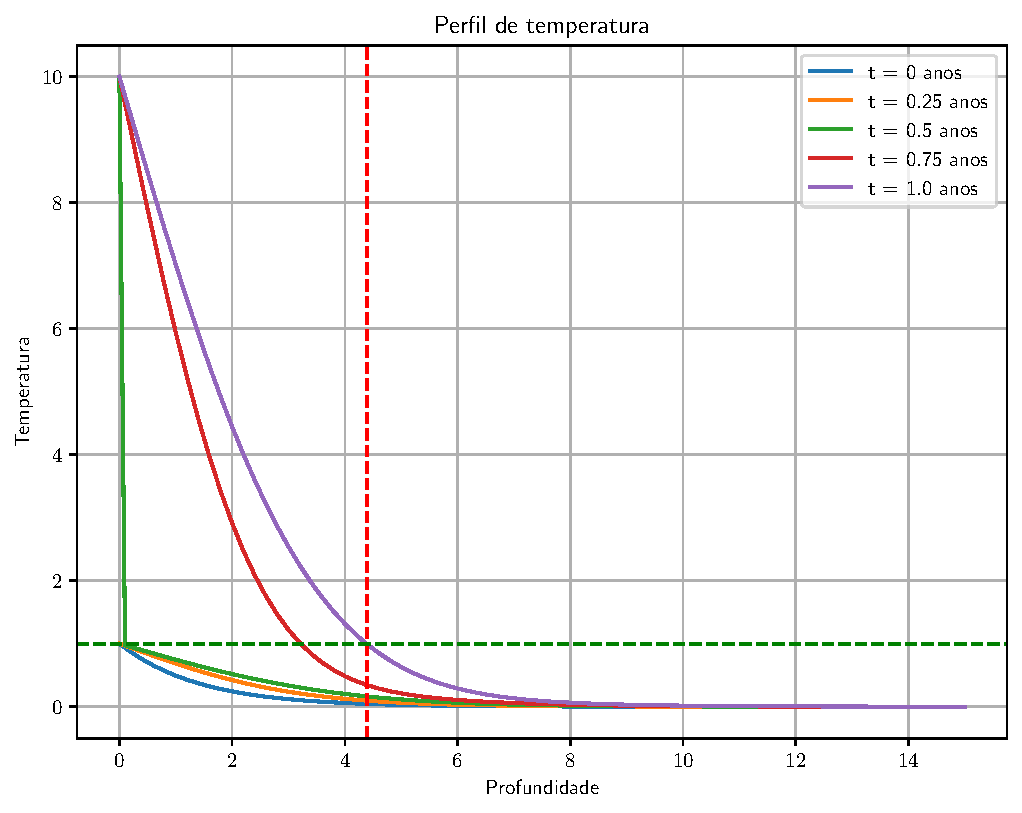
\includegraphics[width=.9\textwidth]{../Report/Codes/exp-euler.pdf}
\end{frame}
%

%
\begin{frame}{Método de Euler explícito --- ordem}
    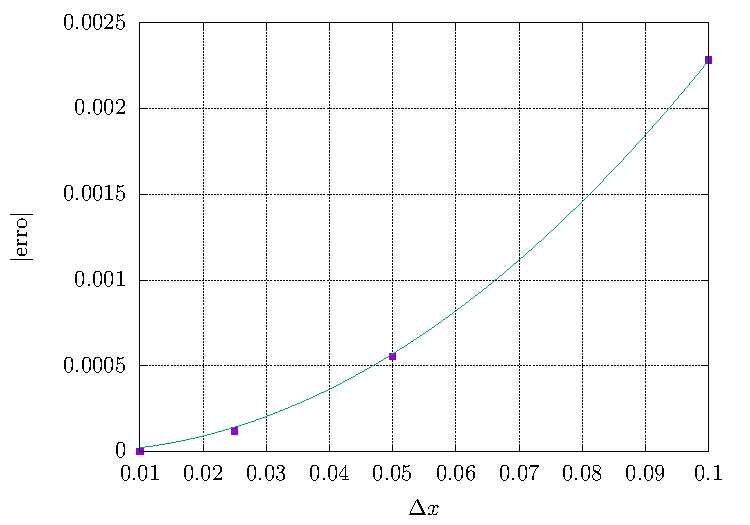
\includegraphics[width=\textwidth]{../Report/Codes/ordem-exp-euler.pdf}
\end{frame}
%

%
\begin{frame}{Método de Crank-Nicolson}
    O método é dado por
    %
	\begin{equation*}
		\label{eq:crank-nicolson}
		-\alpha u^{n+1}_{\ell + 1} + (1 + 2\alpha)u^{n+1}_{\ell} - \alpha u^{n+1}_{\ell - 1}
		= \alpha u^{n}_{\ell + 1} + (1 - 2\alpha)u^{n}_{\ell} + \alpha u^{n}_{\ell - 1}
	\end{equation*}
	%
	com $\alpha = \kappa\mu/2$. Ele é implícito, incondicionalmente estável
    e consistente (logo convergente pelo Teorema de Equivalência de Lax).

    A implicitude do método nos obriga a resolver um sistema linear a cada iteração,
	dado por
	\begin{equation*}
		\begin{bmatrix}
			1 + 2\alpha & -\alpha & 0 & \cdots & 0 \\
			-\alpha & 1 + 2\alpha & -\alpha & \ddots & \vdots \\
			0 & -\alpha & 1 + 2\alpha & \ddots & 0 \\
			\vdots & \ddots & \ddots & \ddots & -\alpha \\
			0 & \cdots & 0 & -\alpha & 1 + 2\alpha
		\end{bmatrix}
		\begin{bmatrix}
			u_1 \\
			u_2 \\
			u_3 \\
			\vdots \\
			u_{N-1} \\
			u_N
		\end{bmatrix}
		=
		\begin{bmatrix}
			b_1 \\
			b_2 \\
			b_3 \\
			\vdots \\
			b_{N-1} \\
			b_N
		\end{bmatrix},
	\end{equation*}
	sendo $N$ a quantidade de pontos na malha espacial.
\end{frame}
%

%
\begin{frame}{Método de Crank-Nicolson --- o algoritmo de Thomas}
    Seja
	%
	\begin{equation*}
		\begin{bmatrix}
			b_1 & c_1 &     &        &  \\
			a_2 & b_2 & c_2 &        &  \\
			    & a_3 & b_3 & \ddots &  \\
			    &     & \ddots & \ddots & c_{n-1} \\
			    &     &  & a_n & b_n 
		\end{bmatrix}\begin{bmatrix}
			x_1 \\
			x_2 \\
			x_3 \\
			\vdots \\
			x_n
		\end{bmatrix} = \begin{bmatrix}
			d_1 \\
			d_2 \\
			d_3 \\
			\vdots \\
			d_n
		\end{bmatrix}
	\end{equation*}
	%
	um sistema linear tridiagonal. O método de Thomas resolve tais sistemas em $\mathcal{O}(n)$
	operações. Este algoritmo não é estável para o caso geral. Não obstante, para Crank-Nicolson
    temos $b_i = 1 + 2\alpha$,
	$a_i = c_i = -\alpha$ e a matriz do sistema é estritamente diagonalmente dominante,
    garantindo estabilidade.
\end{frame}
%

%
\begin{frame}{Método de Crank-Nicolson --- o algoritmo de Thomas}
	A primeira etapa do método consiste de uma varredura para o cômputo de novos coeficientes $c_i'$ e $d_i'$ dados por
	%
	\begin{equation*}
		c_i' = \begin{cases}
			\displaystyle{\frac{c_i}{b_i}}, \ i = 1 \\
			\displaystyle{\frac{c_i}{b_i - a_i c_{i-1}'}}, \ 2 \leq i \leq n-1
		\end{cases}
	\end{equation*}
	%
	e
	%
	\begin{equation*}
		d_i' = \begin{cases}
			\displaystyle{\frac{d_i}{b_i}}, \ i = 1 \\
			\displaystyle{\frac{d_i - a_i d_{i-1}'}{b_i - a_i c_{i-1}'}}, \ 2 \leq i \leq n
		\end{cases}
	\end{equation*}
	%
	Calculados os novos coeficientes, a solução é dada por
	%
	\begin{align*}
		x_n &= d_n' \\
		x_i &= d_i' - c_i' x_{i+1}, \ i = n-1, n-2, \dots, 1.
	\end{align*}
	%
\end{frame}
%

%
\begin{frame}{Método de Crank-Nicolson --- resultados}
    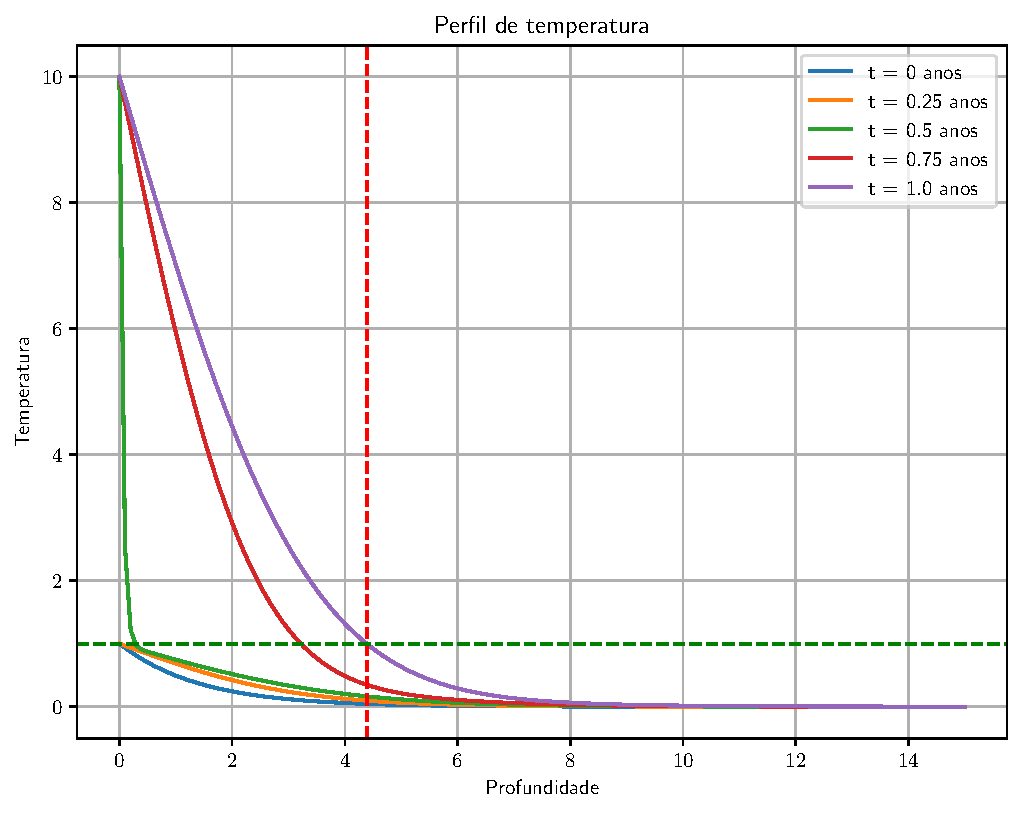
\includegraphics[width=0.9\textwidth]{../Report/Codes/crank-nicolson.pdf}
\end{frame}
%

\begin{frame}{Uma variação do problema}
    Queremos resolver
    %
    \begin{equation*}
        \begin{cases}
			u_t = {(\kappa(x)u_{x})}_x, \ 0 \leq x \leq L, t\geq 0 \\
			u(x,0) = f(t)e^{-q_1x} \\
			u(0,t) = f(t) \\
			u(L,t) = 0
		\end{cases}
    \end{equation*}
    %
    com $q_1 = 0.71\text{m}^{-1}$, $\kappa(x) = {(6.3 + x)}^{\alpha}$ e
    %
    \begin{equation*}
        f(t) = \begin{cases}
			T_w, \ 0 \leq t < 1/2 \\
			T_s, \ 1/2 \leq t \leq 1,
		\end{cases}
    \end{equation*}
    %
    com $T_s > T_w$.
\end{frame}
%

%
\begin{frame}{Volumes finitos}
    Para integrar esta equação, lançamos mão de um método de volumes finitos: para cada iteração na malha espacial,
	tomamos
	%
	\begin{equation*}
		\overline{\kappa}_i = \frac{1}{2}\left( \kappa(x_{i}) + \kappa(x_{i-1}) \right)
	\end{equation*}
	%
	e aplicamos o método de Euler com $\overline{\kappa}_i$.
    Consideramos o mesmo domínio dos métodos anteriores.
	Para que o método convergisse, fixamos $\Delta x = 0.1$ e tomamos
	$\Delta t$ suficientemente pequeno para que
	%
	\begin{equation*}
		\frac{\Delta t}{\Delta x^2} \leq \frac{1}{2\kappa_{\max}},
	\end{equation*}
	%
	com $\kappa_{\max} = {(6.3 + x_{\max})}^{\alpha} = 21.3^{\alpha}$.
\end{frame}
%

%
\begin{frame}{Volumes finitos --- resultados}
    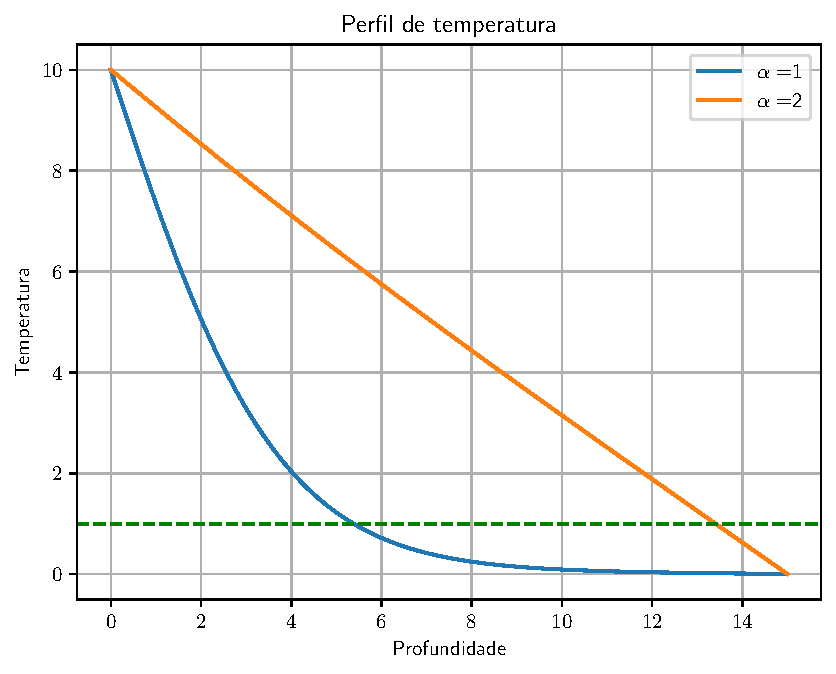
\includegraphics[width=0.9\textwidth]{../Report/Codes/FVM.pdf}
\end{frame}
%

%
\begin{frame}{Referências}
%
\begin{thebibliography}{10}

    \bibitem{Sturm-Liouville}
    \alert{C.C. Lin, L.A. Segel}
    \newblock~{\textit{Mathematics Applied to Deterministic Problems in the Natural Sciences}}
    \newblock~{\textcolor{lightgray}{\textbf{Society for Industrial and Applied Mathematics, 1998}}}

    \bibitem{notas-aula-IMCEDO}
    \alert{Y.D. Sobral}
    \newblock~{\textit{Notas de aula do curso de Introdução a Métodos Computacionais 
    em Equações Diferenciais Parciais}}
    \newblock~{\textcolor{lightgray}{\textbf{Notas de aula, Novembro 2023}}}

    \bibitem{iserles2008}
    \alert{A. Iserles}
    \newblock~{\textit{A First Course in the Numerical Analysis of Differential Equations}}
    \newblock~{\textcolor{lightgray}{\textbf{Cambridge University Press, 2nd edition, 2008}}}
    
\end{thebibliography}
%
\end{frame}
%
\begin{frame}{}
    \centering \Huge
    Obrigado!
    \vfill
    % \includegraphics[width=0.8\textwidth]{Relatório/Figuras/CordaProblem.pdf}
    \vfill
    \usebeamerfont{title} \href{https://github.com/CaioTomas/Trabalho-IMCEDP}{Códigos}
\end{frame}
%
\end{document} % chktex 17